% !TeX spellcheck = en_US
\documentclass[11pt, fleqn, titlepage]{article}
%\usepackage{siunitx}
\usepackage{texfiles/SpeedyGonzales}
\usepackage{texfiles/MediocreMike}
\newcommand{\so}[2]{{#1}\mathrm{e}{#2}}
% \geometry{top=1cm}
\usepackage{hyperref}
\usepackage{ragged2e}
\usepackage{booktabs}
\hypersetup{
	colorlinks=true,
	linkcolor=blue,
	filecolor=magenta,      
	urlcolor=cyan,
}
\title{Phosphate in soil and the effect on barley production}
\author{Oskar Eiler Wiese Christensen s183917 \\ Anders Henriksen s183904 \\ \\ 02445 Project in Statistical Evaluation of Artificial Evaluation}
\date{\today \vspace{2.5cm} \section*{\small Summary} 
%\textit{The summary should contain a summary of the problem that  you are working with, which results you got, as well as main conclusions. \\ Don’t get into technical details. The summary should not be very long} \\
%Purpose and importance of the research
%What has been done
%What has been found
%Implications of the research
\justify{\footnotesize Farmers will need more effective agriculture as the population grows. This can be accomplished by optimizing the amount of bioavailable phosphorous in the soil. The purpose of this paper is to analyze two different measurements of phosphorous in the soil. The measurements are Olsen P and DGT. Furthermore, it is studied which measurement is better at describing the yield. A linear and non-linear Michaelis-Mentel model have been fit to the data to find the best possible measurement to use, and ANCOVA has been applied for finding the significance of phosphorous for the yield. These analyses have shown that DGT is the best of the two measurements and that phosphorous has a remarkably significant influence on the harvest yield. This shows that phosphorous measurements can be constructive in helping farmers estimate the yield. Meanwhile, when estimating this, DGT is the better of the measurements, though it also costs more, so farmers should take into consideration the cost-benefit of using DGT instead of Olsen P.}}

\pagestyle{plain}
\fancyhf{}
\rfoot{Page \thepage{} of \pageref{LastPage}}

\graphicspath{{Billeder/}}

\begin{document}

\maketitle
%\thispagestyle{fancy}
%\tableofcontents

\section{Introduction}
% \textit{Briefly introduce the background and setting of the problem, as well as the aim of the report. Furthermore, you could give a very short description of the analysis that will be applied.} \\ \\
The world is overpopulating. The population has grown exponentially over time while the surface of earth has naturally stayed constant. People have ever increasing problems with allocating enough space for agriculture. This will undoubtedly lead to huge agricultural problems, especially underproduction. One way to solve this issue could be to get a larger amount of cultivated land, which is not an effective long term solution as the population grows and the skirmish for satisfying the nutritional needs becomes ever larger. The other option is to get more bang for your buck, or in other terms, getting a bigger yield from the same amount of land. There are many different ways of accomplishing this, but one would be to make sure to have large amounts of unbounded phosphate in the soil of the farmland, as this is a necessary nutrient for plant growth. Two possible measurements for this phosphorous amount are Olsen P and the newer, although more expensive, DGT measures. 

One natural and important question for farmers, which will be uncovered in this paper, is whether one measure is significantly different than the other and which measure is best, which will be determined by finding the measure with the lowest error on a non-linear fit to the data. Meanwhile, another interesting question for this paper is if the phosphorous amount even has a significant influence on the yield of the farms, which can be uncovered by a simple use of ANCOVA. The hypothesis prior to the carrying out of the experiments is that DGT should be a better measurement for determining the amount of bioavailable phosphorous is the soil, as this method is both more expensive and newer. Meanwhile, it is expected that the amount of bioavailable phosphorous should have a significant effect on the yield, as more plant nutrients should lead to bigger and stronger plants.

\section{Data}
%\textit{Describe of the data you are analyzing. What kinds of data do you have, how were they collected (if applicable)? \\ Include a few good plots to highlight important features in data. You can put additional plots in the appendix.}\\
\noindent
The data consists of soils samples that were obtained from fields in Denmark and Norway respectively. Each field was divided into smaller subfields (plots), and barley was then sown on each of the subfields. By doing so, variation between fields is eliminated, and thus a number of variables affecting plant growth is avoided. The only variation that is interesting for this study is the amount of phosphorus in the soil. On each of the subfields, a soil sample was obtained and analyzed for bio-available phosphorus using two methods, Olsen-P and DGT. Where Olsen-P is the traditional method and DGT is a newer and more expensive method. The data consists of four different variables; Location, yield, DGT measurement and Olsen-P measurement, as well as 36 different observations, 4 from each location except for location 9, where two of the yield measurements are missing. Location is a factor, while every other variable is continuous.
\\ \noindent 
Since both olsen-P and DGT is a measurement for the yield, it would be suspected that there is a correlation between both of the measurements. 
\begin{figure}[H]
	\centering
	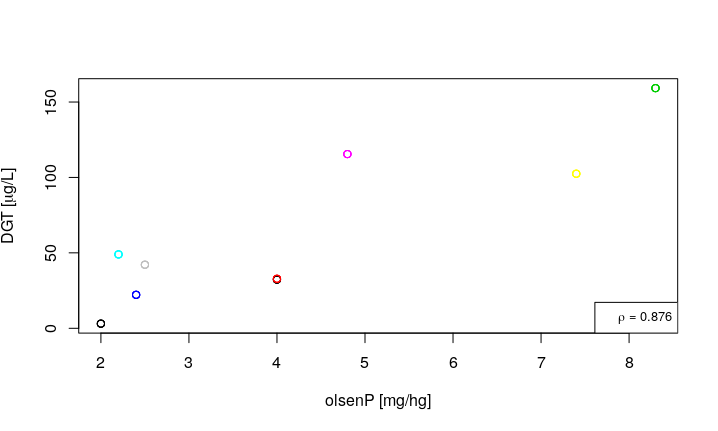
\includegraphics[width=0.7\linewidth]{billeder/dgtolsencor.png}
	\caption{Scatterplot of the DGT and olsenP measurement. The pearson correlation $ \rho $ is calculated and shows a strong relationship between the two measurements.}
	\label{fig:dgtolsencor}
\end{figure}
\noindent It is seen from \ref{fig:dgtolsencor} that olsenP and DGT are indeed correlated. Hence, they both describe the same thing, but since the correlation is not 1, the two measurement techniques do differ. This difference will be investigated in this project. To get an understanding of how yield is expressed in terms of DGT and Olens P values, the yield over DGT and yield over Olsen P plots are shown below, figure \ref{fig:measurementz}. 


\begin{figure}[H]
	\centering
	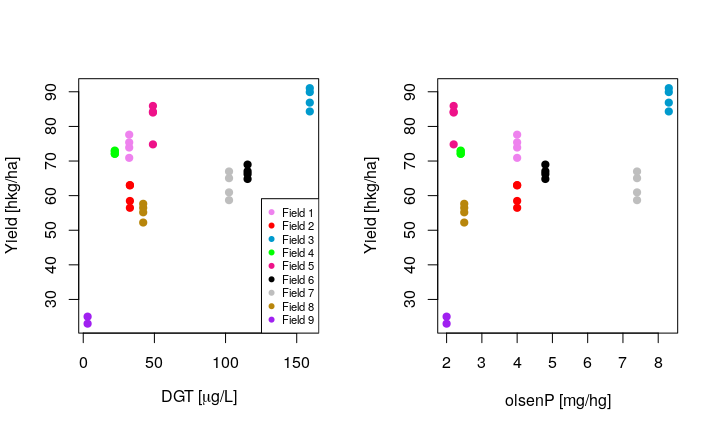
\includegraphics[width=0.7\linewidth]{billeder/measurementz}
	\caption{Scatter plot of the yield against measurements. On the right is a plot of the yield against the DGT measruement. On the left is a plot of the yield against the olsenP measurement.}
	\label{fig:measurementz}
\end{figure}

In figure \ref{fig:measurementz}, it is clear that low values of both DGT and Olsen P leads to a low yield, while somewhat higher values of DGT and Olsen P do not lead to much higher values of yield. This could suggest that the Michaelis-Menten model could be effective for fitting this data. This will be uncovered in the sections below.

\section{Methods}
%\textit{Describe the methods you used and why you decided to use them. Also discuss the assumptions behind the methods. Do not go into detail with theory.}\\\\ 
To make a relevant recommendation for farmers in order to choose between the two measurements DGT and olsenP, the data for the measurements respectively is fitted to both a linear model and a non-linear model. To investigate wheter the amount of bioavailable phosphorous influence the harvest yield an analysis of covariance is conducted.

\subsubsection*{Linear Regression}
In linear regression, a model is fitted to the data. In regression the model that is to be constructed tries to fit the parameters a and b, that makes the data most likely.

\[ y \approx a \cdot x + b, \quad x \in \mathbb R  \]

\noindent
In linear regression the response and explanatory variable are both continuous. The optimal parameters for the linear fit are estimated by the maximum likelihood. That is, to minimize the sum of squares of the residuals. \cite{statbog} 

\subsubsection*{Non-linear Regression}
The second type of regression used to determine the measurement that best describes the yield is non-linear regression, which in this case was carried out using the Michaelis-Menten model, shown below.

\[y \approx \frac{\alpha \cdot x}{\beta + x}, \quad x > 0 \]

The reason for choosing the Michaelis-Menten model as a non-linear fit is due to the fact that this model has been demonstrated to effectively describe this type of data. 

\subsubsection*{Analysis of Covariance: ANCOVA}
Analysis of covariance involves a combination of linear regression and analysis of variance(ANOVA). The response variable is continuous and at least one of the explanatory variables is continuous, while at least one other explanatory variable is categorical. The ANCOVA evaluates if the means of the response variable is equal across the categorical explanatory variable. The reason for using ANCOVA is due to the analysis ability to determine if the explanatory variables are significant in describing the response variable. In the scope of this project the analysis can discover if both of the measurements significantly, with $ \alpha = 0.05 $, influence harvest yield and thereby determining if the amount of bioavailable phosphorous influence the harvest yield. Therefore, two separate Ancova are made. One with DGT as an explanatory variable and one with olsenP as an explanatory variable.   \cite{statbog} 


\section{Results}
%\textit{Present the results. \\ Tables and figures are good ways of illustrating results.}

To uncover which measurement best describes the yield, the linear fits of the yield over DGT and yield over olsen P with accompanying $r^2$-values are shown below.

\begin{figure}[H]
	\centering
	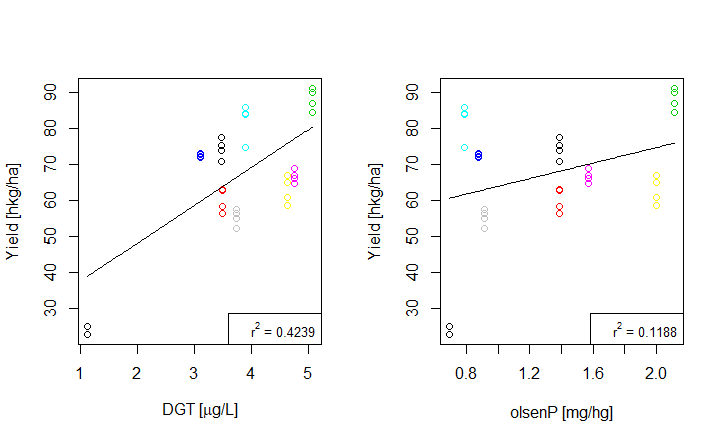
\includegraphics[width=0.6\linewidth]{billeder/Linearfit.png}
	\caption{A linear regression of the yield against the DGT and OlsenP measurements respectively. On the left the DGT-measurement with a $ r^2 = 0.42 $. On the right the OlsenP measurement with a $ r^2 = 0.12 $.}
	\label{fig:linearfit}
\end{figure}

\noindent The non-linear Michaelis-Menten fits of the yield over DGT and yield over olsen P with accompanying MSE-values are also shown below.

\begin{figure}[H]
	\centering
	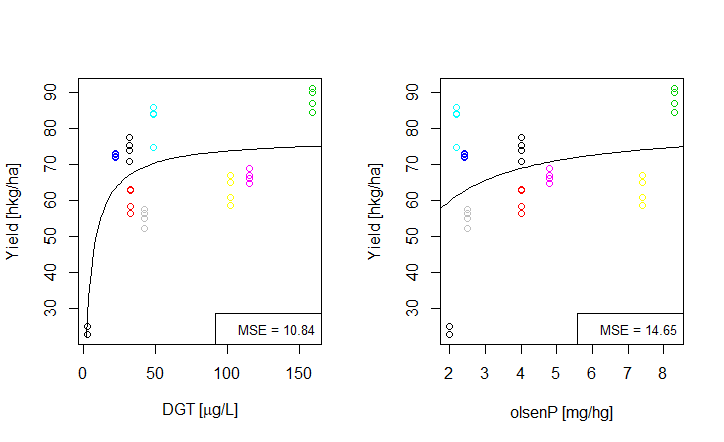
\includegraphics[width=0.6\linewidth]{billeder/non-linearfit.png}
	\caption{A non-linear Michaelis-Menten fit of the yield against DGT and OlsenP respectively. The MSE of the two fits are compared, where MSE for the DGT is $ MSE = 10.84 $ and the MSE for OlsenP is $ MSE = 14.65 $.}
	\label{fig:non-linearfit}
\end{figure}

\noindent To investigate if the amount of bioavailable phosphorous has a significant influence on the yield, an ANCOVA is performed with yield as the response variable and Olsen P, DGT and location as the explanatory variables. This yields the following p-values for the explanatory variables.

\begin{table}[H]
	\centering
	\begin{tabular}{l r}
		\toprule
		Variable     & p -value                       \\ \midrule
		DGT          & $3.931 \cdot 10^{-13}$       \\ 
		Olsen P      & $1.715 \cdot 10^{-10}$        \\ \bottomrule 
	\end{tabular}
	\caption{Table of \textit{p}-values for each of the ANCOVA models.}
	\label{tabel}
\end{table}

\section{Discussion}
%\textit{What do your results show? \\ Discuss your results. How reliable are they?}

\subsection*{What does the results show?}
The linear regression fit shows, that the DGT measurement has a higher coefficient of determination than the olsenP measurement. As for the michalis-menten regression, the DGT measurement, has a lower mean squared error than olsenP. From \ref{fig:linearfit} and \ref{fig:non-linearfit} the coefficients that makes the DGT-data most likely describes the yield better than the coefficients that makes the olsenP-data most likely. Thus, one could use this as an argument for recommending the DGT-measurement over the olsenP-measurement. Another question that could be raised is, if the DGT measurement describes the yield significantly more effectively than the olsenP measurement.

\subsection*{OlsenP or DGT?} 
% How reliable are the reults 
From the p-values seen in table \ref{tabel} from the ANCOVA, both DGT and OlsenP are significant with $ \alpha = 0.05 $, which shows that both types of measurements have a significant description of yield. From the two type of regressions, it is seen that data from the DGT measurements has a better description of the yield. Due to the limitation of the data there is no way to tell if the DGT measurement is statistically better than olsenP. However, DGT has higher coefficient of determination in the linear regression and lower MSE in the michales-menten fit. On the other hand, the DGT measurement is more expensive than the traditional olsenP measurement and with no way to statistically test if one is better than the other the farmers should take into consideration the cost-benefit of using the DGT over Olsen P. 

\subsection*{Exploration of the cost-benefit }
A way to determine if its worth investing in the DGT measurement would be to conduct a new experiment. The experiment would be very similar to the one in this project, where additional variables would be included. This would be the revenue of the barley, the quality, the amount of barley etc. Through this data, one would be able to also determine if it would be beneficiary for the farmer to invest in a newly developed measurement such as DGT. Furthermore, the experiment would allow for more data on the DGT and OlsenP measurements which might enable a way to tell if there is a significant difference between them. Moreover, a paired t-test can be performed on the new DGT measurement to tell if the description of the yield is consistent, or if the data from this particular experiment happens to randomly describe the yield well. 


\section{Conclusion}
%\textit{What are your conclusions? The conclusion should be connected to the aim of the report in the introduction. \\ Highlight important results \\ If you have found interesting problems/aspects that you haven’t carried out, you can specify them here as ‘future work’.}

The purpose of this project has been to determine whether the DGT measurement is significantly better then OlsenP and if the amount of bioavailable phosphorous has an influence on the harvest yield. To uncover the truth, the MSE of the non-linear fit of the yield against DGT and OlsenP respectively showed that DGT has a lower MSE. Thus, DGT-measurement describes the yield better than the OlsenP. However, there is no way to tell if DGT is significantly better than OlsenP. Furthermore, the analysis of covariance shows that both of the measurements describes the yield at $ 0.95 $ level of significance. The ANCOVA also reveals that the amount of bioavailable phosphorus indeed does influence the harvest yield. In conclusion, using DGT over OlsenP is only a cautious recommendation due to the fact that there is no way to tell if one of the measurements are significantly better than the other. Since the DGT is more expensive than the traditional OlsenP measurement an analysis of the cost-benefit as well as more data would yield a more precise conclusion and guidance to the farmers who need the knowledge of the efficiency of the two measurements. This will be left as future work for new papers to come.

\newpage

\bibliographystyle{IEEEbib}
\bibliography{refs}


\end{document}
